\chapter{Automi a Pila}
Gli automi a pila (PDA - Push Down Automa) sono una settupla definita come segue
\begin{equation*}
    A={Q, \Sigma, \Gamma, \delta, q_0, Z_0, F}
\end{equation*}
Dove:
\begin{itemize}
    \item $Q$ è un insieme di stati
    \item $\Sigma$ è un alfabeto
    \item $\Gamma$ è un alfabeto di simboli di stack
    \item $\delta \in Q x (\Sigma \cup \{\epsilon\}) x \Gamma \rightarrow P(Q x \Gamma)$ 
    \item $q_0$ è lo stato iniziale
    \item $Z_0$ simbolo inizialmente presente sulla pila
    \item $F$ è l'insieme di stati finali
\end{itemize}
La definizione è non deterministica.
La pila costituisce una memoria di lavoro che utilizzeremo per memorizzare simboli a nostri piacimento
(vedremo che sarà fondamentale per poter riconoscere i CF Language).
\paragraph{Osservazione}Ci deve essere sempre un simbolo sulla pila, altrimenti l'automa si blocca, l'unico caso in
cui la pila è vuota è quando l'automa accetta per pila vuota.
\section{Accettazione per stato finale o pila vuota}
Possiamo costruire due tipi di PDA
\begin{itemize}
    \item PDA che accettano per pila vuota
    \item PDA che accettano per stato finale
\end{itemize}
\section{PDA Deterministici VS Non Deterministici}
Nel caso di \textbf{PDA non deterministici} vedremo che entrambe le tipologia hanno la stessa potenza,
discorso diverso per i \textbf{deterministici}, dato che questi ultimi \textbf{non sono in grado di riconoscere tutti i CF Language},
oltretutto posso costruire un automa che accetta per pila vuota solamente nel caso in cui il linguaggio
considerato goda della \hyperref[sec:Prefix-Free]{proprietà del prefisso}.
Quindi i NPDA sono più potenti dei DPDA (è stata spiegata la dimostrazione).

%Inserire dimostrazione

\paragraph*{Osservazione} Se $L\in Reg$ allora $\exists PDA$ (non deterministico)
tale che $L=L(P)$ accettato per stati finali, inoltre $\exists PDA P_n$ non deterministico tale che 
$L=N(P_n)$ accettato per pila vuota. Infatti un PDA non deterministico è un $\epsilon$-NFA che usa una pila.
\\ Non è detto però che $\exists$ DPDA $P_N$ tale che $L=N(P_n)$.
\\\textbf{Per pila vuota i DPDA sono meno potenti dei DFA} 
non riescono ad accettare tutti i linguaggi CF e neanche tutti i Linguaggi Regolari!
Per esempio il linguaggio $L_{vv^r} = \{ww^r | w \in {0,1}*\} \in$ CFL, non è accettato
da DPDA, mentre viene accettato da NPDA. Questo perchè in questo caso il DPDA non riesce
a capire quando iniziare a svuotare la pila, inserendo però un "segnale di mezzo" c $\{wcw^r\}$
che fa capire all'automa quando iniziare a svuotare la pila allora si può creare un DPDA, quando legge c
cambia stato e iniziare a svuotare la pila.
\section{Descrizioni Istantanee - ID}
Una ID (o configurazione) è una tripla (q, w, $\gamma$) dove:
\begin{itemize}
    \item $q \in Q$ è lo stato attuale
    \item $w \in \Sigma^*$ è l'input residuo (ciò che resta da leggere)
    \item $\gamma \in \Gamma^*$ è il contenuto attuale della pila
\end{itemize}
Attverso le ID possiamo rappresentare i vari stati del PDA per arrivare a
mostrare l'intera esecuzione del PDA (anche i casi dove si blocca).
\section{Linguaggi accettati dai PDA}
I PDA  
\section{Proprietà del prefisso - Prefix-Free Language}
\label{sec:Prefix-Free}
Un Linguaggio L ha la proprietà del prefisso (cioè è Prefix Free) se $\nexists x,y \in L$ tali che $x \neq y$ e $x$
è prefisso di $y$. 
\paragraph*{Teorema} Un linguaggio L è $N(P)$ (accetta per pila vuota) per un DPA
se e solo se L gode della proprietà del prefisso (cioè è prefix-free) ed è $L(P')$
Come già riportato a inizio paragrafo, utilizzo questa proprietà per verificare se posso
costruire un DPDA che accetta per pila vuota o se sono costretto ad accettare per stato
finale.
\paragraph*{Esempio} Il linguaggio denotato dalla Espressione Regolare (ER) $\{0\}*$ non è prefix-free
quindi non posso costruire un DPDA che accetti per pila che lo riconosca.
\paragraph*{I DPDA che accettano per pila sono meno potenti di quelli che accettano per stato finale} perchè accettano
una sottoclasse di linguaggi che vengono accettati per stati finali (quelli appunto Prefix-Free).
\subsection*{Dimostrazione}Ho un DPDA P che accetta per pila vuota, suppongo che
L=N(P) e per assurdo supponiamo che L non sia prefix-free.
\\ Allora $\exists x,y \in L$ t.c $x \neq y$ e $x$ è prefissa di $y$.
\\ Pongo $y = xw$, se P accetta x dopo aver consumato x, la pila è vuota (dato che x è prefissa di y).
\\ P però non può accettare y anche se $y \in L$ perchè dopo aver consumato x la pila è vuota e dato che
il PDA è deterministico e x è prefissa di y l'automa nel leggere y rifarà gli stessi passi di x e quindi
arriverà a svuotare la pila prima di aver consumato tutta la stringa.
\paragraph*{Riassumendo}Per pila vuota i DPDA non sono in gradi accettare tutti i CFL e neanche tutti i LR.
\section{Riassunto Linguaggi riconosciuti dai PDA}
PDA senza D iniziale significa non deterministici.
\begin{center}
    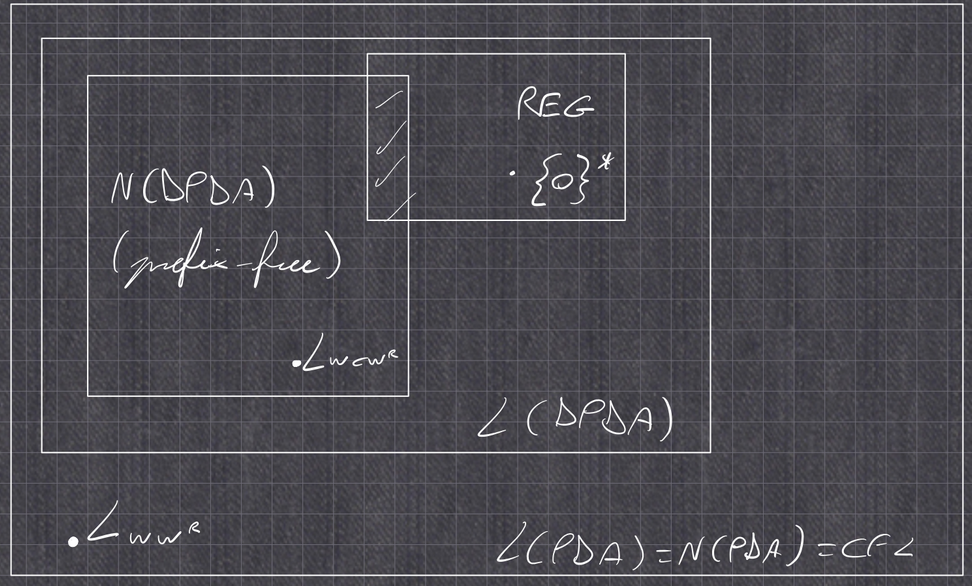
\includegraphics[width=120mm, scale=0.5]{pda_linguaggi_accettati.png}
\end{center}

